\documentclass[%
12pt, %
final, % 
oneside, % 
onecolumn, %  
centertags]{article} % относится к классу article и размер шрифта 12 пунктовб, {article: статья, report: отчеты и диссертации, book: книга, letter: письмо}

% ------ page construction 

\topmargin= -30pt % насколько сверху будет страница
\textheight= 650pt

% ------ Пакеты расширения

\usepackage[utf8]{inputenc} % задает кодировку, utf-8 кодировка, включающая в себя знаки почти всех языков мира
\usepackage[english, russian]{babel} % подключает необходимые языки, основным языком является английский
\selectlanguage{russian} % настройки будут на английском, но писать будет на русском

\usepackage{euscript}
\usepackage{supertabular}

\usepackage[colorlinks=true,linkcolor=black,unicode=true,urlcolor = blue]{hyperref} %hypered
\usepackage[pdftex]{graphicx} % для графики

\usepackage{amsthm, amssymb, amsmath, amsfonts} % математический пакет, математические шрифты
\usepackage{textcomp}
\usepackage[noend]{algorithmic}
\usepackage[ruled]{algorithm}
\usepackage{lipsum}
\usepackage{indentfirst}
\usepackage{babel}
\usepackage{pgfplots}
\usepackage{setspace}
\usepackage{xcolor}
\usepackage{hyperref}

\linespread{1.2} 
\setlength{\parindent}{2.4em}
\setlength{\parskip}{0.1em}

\pgfplotsset{compat=1.9}
\pgfplotsset{model/.style = {blue, samples = 100}} 
\pgfplotsset{experiment/.style = {red}}

\theoremstyle{plain}
\binoppenalty=10000

\newtheorem{theorem}{Теорема}[section] % theorem

\theoremstyle{definition}
\newtheorem{definition}{Определение}[subsection]

\theoremstyle{remark}
\newtheorem{remark}{Замечание}[section]

\newtheorem{corollary}{Следствие}

\newtheorem{solution}{Решение}

\newtheorem{proposition}{Proposition}

\newtheorem{example}{Пример}

\newtheorem{lemma}{Лемма}[section]

\renewcommand*{\proofname}{Proof}

\graphicspath{ {./image/} }

\usepackage{enumitem}
\begin{document}

\begin{titlepage} 
\begin{center}
\textbf{}\\[10.0cm]
\textbf{\LARGE Страхование и актуарная математика}\\[0.5cm]
\textbf{\Large Test 2 Try 1 17.12.2020} \\[0.2cm]


\begin{center} \large
{Преподаватель:} \\[0.5cm]
\textsc {Радионов Андрей Владимирович}\\
\end{center}

\vfill 



{\large {Александр Широков, ПМ-1701}} \par
{\large {Санкт-Петербург}} \par
{\large {2020 г., 7 семестр}} 

\end{center} 
\end{titlepage}

\newpage

\begin{enumerate}
\setlength\itemsep{-0.15em}

\item В модели коллективного риска, где количество убытков определяется Пуассоновской случайной величиной, функция распределения суммарного ущерба в точке ноль:
\begin{enumerate}
\setlength\itemsep{-0.15em}
    \item делает скачок;
    \item непрерывна;
    \item не определена;
    \item ни одно из вышеперечисленных утверждений не является всегда верным.
\end{enumerate}

\textbf{Решение:}

в модели индвидуального риска она точно делает скачок. Здесь мне кажется, зависит от производящей функции моментов ущерба, поэтому отвечу, что $d$.

\item Рассматривается модель, в которой с вероятностью $p$ реализуется один ущерб, а с вероятностью $(1-p)$ два ущерба. Ущербы независимы и определяются нормальными случайными величинами с ожиданием 5 и дисперсией 1. Плотность распределения общего убытка приведена на рисунке. Тогда:

\begin{figure}[!h]
    \begin{center}
    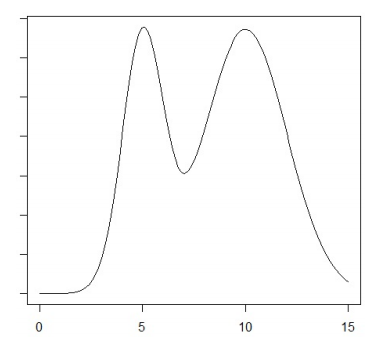
\includegraphics[scale=0.5]{image/1.png}
    \end{center}
\end{figure}


\begin{enumerate}
\setlength\itemsep{-0.15em}
    \item $p>0.5$;
    \item $p<0.5$;
    \item $p=0.5$;
    \item ни одно из вышеперечисленных утверждений не является всегда верным.
\end{enumerate}

\textbf{Ответ:} $p<0.5$. Общая плотность имеет вид $p$ умноженное на плотность нормальной величины с параметрами $N(5, 1)$ + $(1-p)$ умноженное на плотность суммы случайных величин, которая для нормальных распределений равна $N(5 + 5, 1^2 + 1^2) = N(10, 2)$. Тяжело даются пока такие задания.

\item Рассматривается источник риска, ущерб по которому возникает с вероятностью 0.1. В случае возникновения размер ущерба определяется случайной величиной с плотоностью $f_\xi(x)=ax^2,$ $x\in[0;10].$ В противном случае ущерб равен нолю. Найти функцию распределения ущерба и дисперсию ущерба.

\textbf{Решение:}

Вероятность отсутствия ущерба $p = 0.9$. Найдём плотность распределения ущерба:
$$f_{\eta}(x) = (1-p)f_{\xi}(x) = 0.1 \cdot ax^2, x \ \in [0;10]$$

Из этого выражения мы можем найти математическое ожидание ущерба:
$$E(\eta) = \int\limits_{0}^{10} 0.1 \cdot ax^2 \operatorname{dx} = 33.33 \cdot a$$

И теперь найдём дисперсию ущерба:
$$D(\eta) = \int\limits_{0}^{10} (x - E(\eta))^2 \operatorname{dx} = \int\limits_{0}^{10} (x - 33.33 \cdot a)^2 \operatorname{dx} = 11111a^2 - 3333.33a + 333.333$$

Найдем функцию распределения из следующих формул:
$$F_{\xi}(x) = \frac{F_{\eta}(x) - p}{1-p}$$
$$F_{\eta}(x) = F_{\xi}(x) \cdot (1 - p) + p = a \cdot \frac{x^3}{3} \cdot 0.1 + 0.9 = 0.3ax^3 + 0.9 \eqno \blacksquare$$

\item Рассматривается модель коллективного риска $S_{coll}=\sum\limits_{i=1}^N\xi_i,$ где производящая функция вероятностей числа убытков есть $\phi(z)=\left(\dfrac{0.5z}{1-0.5z}\right)^5,$ а производящая функция моментов $\xi_i$ есть $\psi_{\xi_i}(t)=(1-2t)^{-2.5}.$ Найти $P(N=0),$ $P(N=1),$ $E\xi_i,$ $DS_{coll}.$

\textbf{Решение:}

Найдём производящую функцию моментов коллективного риска:
$$\psi_{S_{coll}} = \phi_{N}\left(\psi_{\xi_i}(t)\right)$$

не стал подставлять одно в другое.

Чтобы найти математическое ожидание (а затем и диспесию по производящей функции моментов), возьмём производную по $t$ и подставим $0$ в нее. Все действия посчитаны в Wolfram.
$$E\xi_i = \psi_{\xi_i}(t)'_{t=0} = 5$$
$$E\xi_i^2 = \psi_{\xi_i}(t)''_{t=0} = 35$$
$$D\xi_i = E\xi_i^2 - (E\xi_i)^2 = 35 - 25 = 10$$ 
$$D(S_{coll}) = (E(\xi_i))^2 \cdot D(N) + D(\xi_i) \cdot E(N)$$

Здесь мы уже знаем все характеристики, связанные с убытком, поэтому нам необходимы характеристики случайной величины, отвечающей за убыток. Из производящей функции вероятностей найдем следующие величины:
$$P(N = 0) = \frac{\phi^{(0)}(0)}{0!} = 0$$
$$P(N = 1) = \frac{\phi^{(1)}(0)}{1!} = 0$$

Чтобы найти дисперсию и математическое ожидание $N$ получим производящую функцию моментов из производящей функции вероятности, подставим $e^t$ в производящую функцию моментов:
$$\psi_N(t) = \left(\dfrac{0.5 \cdot e^t}{1-0.5 \cdot e^t}\right)^5$$

Найдем математические ожидания и дисперсию и из него дисперсию коллективного риска:
$$E(N) = \psi_N(t)'_{t=0} = 10$$
$$E(N^2)  = \psi_N(t)''_{t=0} = 110$$
$$D(N) = 10$$
$$D(S_{coll}) = (E(\xi_i))^2 \cdot D(N) + D(\xi_i) \cdot E(N) = 25 \cdot 10 + 10 \cdot 10 = 350 \eqno \blacksquare$$



\item 
Выберите верные утверждения:
\begin{enumerate}
\setlength\itemsep{-0.15em}
    \item если обе компоненты вектора возвести в квадрат, соответствующая ему копула не изменится;
    \item если обе компоненты вектора возвести в куб, соответствующая ему копула не изменится;
    \item если обе компоненты вектора возвести в квадрат, соответствующая ему копула может не изменится, но может и измениться;
    \item если обе компоненты вектора возвести в куб, соответствующая ему копула может не изменится, но может и измениться.
\end{enumerate}

\textbf{Ответ:} отвечу, что верным являются ответы $c$ и $d$. Похоже на правду :(.

\item Найти копулу и маргинальные распределения для вектора с совместной функцией распределения $F(x_1,x_2)=\dfrac{x_2^2\sqrt{x_1}/4}{\sqrt{x_1}+x_2^2/4-x_2^2\sqrt{x_1}/4},x_1\in[0;1],x_2\in[0;2].$

\textbf{Решение:}

$$F_{X_1, X_2}(x_1, x_2) = C(F_{X_1}(x_1), F_{X_2}(x_2))$$

Сначала найдем маргинальные распределения по следующим формулам:
$$F_{X_1}(x1) = F_{X_1, X_2}(x_1, x_2 \to \infty) = \frac{\sqrt{x_1}}{1 - \sqrt{x_1}}$$
$$F_{X_2}(x_2) = F_{X_1, X_2}(x_1 \to \infty, x_2) = \frac{x_2^2}{4-x_2^2}$$

Теперь необходимо найти копулу. Чуть перезапишем функцию начальную:
$$F(x_1, x_2) = \frac{1}{\frac{4}{x_2^2} + \frac{1}{\sqrt{x_1}}- 1}$$

Теперь выразим $\sqrt{x_1}$ и $x_2^2$ через маргинальные функции распределения:
$$\sqrt{x_1} = \frac{F_{X_1}(x_1)}{1 + F_{X_1}(x_1)}$$
$$x_2^2 = \frac{4 \cdot F_{X_2}(x_2)}{1 + F_{X_2}(x_2)}$$

Тогда, обозначая наши маргинальные распределения за $u_1$ и $u_2$ получим формулу копулы:
$$C(u_1, u_2) =  \frac{1}{\frac{4}{\frac{4 \cdot u_2}{1 + u_2}} + \frac{1}{\frac{u_1}{1 + u_1}}- 1} \eqno \blacksquare$$


\item Рассматривается двумерный вектор $\zeta,\xi$ с копулой $C(u_1,u_2).$ Найти копулу для вектора $(\vartheta,-\zeta).$

\textbf{Решение:} 

Наверное, имелось ввиду вектора $(\xi, -\theta)$. Так как у нас равномерные распределения на гиперкубе в общем случае $[0,1]^n$, то добавление минуса делает наши распределения на $[0,-1]$. Поэтому в копуле перед $u_2$ необходимо поставить знак минус в этой функции, тогда равномерность на $0,1$ сохранится. Либо тут задача с подвохом, но странно.$\blacksquare$

\item Выберите верные утверждения:
\begin{enumerate}
\setlength\itemsep{-0.15em}
    \item максимум из трёх независимых, одинаково распределенных экспоненциальных случайных величин имеет распределение Гумбеля;
    \item максимум из трёх независимых, одинаково распределенных экспоненциальных случайных величин имеет распределение Вейбулла;
    \item максимум из трёх независимых, одинаково распределенных экспоненциальных случайных величин имеет распределение Фреше;
    \item ни одно из вышеперечисленных утверждений не является верным.
\end{enumerate}

\textbf{Решение:}

Ответ: Мне кажется, что можно доказать, что верный только первый вариант (если останется время, я это сделаю). Вкратце: когда мы запишем функцию распределения в $n$-ой степени получим, что при определённо выбранных константах $a_n$ и $b_n$ сходится к $e^{e^{-x}}$, что является распределением Гумбеля. $\blacksquare$

\item Рассматривается случайная величина $Z=\max(X,Y),$ случайные величины $X,Y$ независимы. Объясните, как класс предельного распределения для $Z$ будет зависеть от классов пределельных распределений для $X$ и для $Y.$

\textbf{Решение:}

У нас есть две независимые случайные величины, следовательно мы можем найти совместную функцию распределения, как произведение соответствующих функций распределения. Так как у нас распределение $Z = \max(X, Y)$, то мы можем найти и функцию этого распределения - $F_{Z}(x) = (F_{X}(x) \cdot F_{Y}(x))^2$. Что мы можем сказать про классы. Если экспоненциальное распределение, то из предыдущего задания предельное распределение - к Гумбелю, максимум из случайных величин с распределением Фреше - к Фреше. Задачка из дз была тоже: проверить, что предельным распределнием к $\max$ из независимых случайных величин Вейбулла стремится к Вейбуллу. При одинаковых классах мы однозначно можем сказать, к какому классу принадлежит, при разных мы особо не проверяли, как мне кажется - предположу, что нужно аналитически проверять. $\blacksquare$

\item Объясните, какие подходы можно использовать для оценки поведения хвостов распределений с помощью теории экстремальных значений.

\textbf{Решение:}

Первый подход заключается в самом определении "тяжёлого хвоста" - это означает, что плотность распределения стремится к оси абцисс медленнее, чем плотность экспоненциального распределения. Поэтому для оценки поведения хвоста в принципе мы можем находить следующий предел:
$$\lim\limits_{x \to \infty} \frac{f_{\xi}(x)}{f_{\eta}(x)}$$
где $f_{\eta}(x)$ является плотностью экспоненциального распределения. Если предел стремится к нулю то хвост распределение с плотностью $f_{\xi}(x)$ убывает быстрее, чем у экспоненциального - не особо тяжёлый. Если к бесконечности - хвост убывает медленее экспоненциального - тяжёлый.

Оценку правого хвоста можно производить, например, параметрически (чем мы занимались в первой половине семестра, оценивая квантилями), но такой подход не очень выгоден - на "подгону параметра распределения" влияют все элементы выборки и старшие квантили с маленькой вероятностью возникновения большого ущерба могут недооцениваться (пример с дамбой). 

Методы, которые были предложены: будем оценивать максимальный ущерб в течение некотора периода на основе выборки из максимальных ущербов. По теореме Фишера-Типпета мы можем понять к какой максимальной области притяжения пренадлежит распределение и понять, насколько тяжёлый хвост (при $\beta > 0$ самые тяжёлые хвосты - распределение Фреше). Хвост можно оценивать и из предела $\lim\limits_{x \to \infty} \frac{L(ax)}{L(x)} = 1, a>0$, где $L(x)$ - медленно меняющаяся функция. Но при этом методе мы много теряем информации - очень много выбрасываем элементов выборки.

Второй подход: выбрать некоторый достаточно большой порог и исследовать распределение ущербов превышающих их. Оценивать поведение хвоста можно по функции распределения за порогом:
$$F_{\xi}(x) = \frac{F_{\eta}(d + x) - F_{\eta}(d)}{1 - F_{\eta}(d)}$$
где $d$ - порог, так и по теореме Balkema-Pickands (извиняюсь). $\blacksquare$.
\end{enumerate}



\end{document}